\subsection{Ядерные оценки плотности распределения}
\label{subsec:result_kde}
\begin{figure}[H]
	\centering{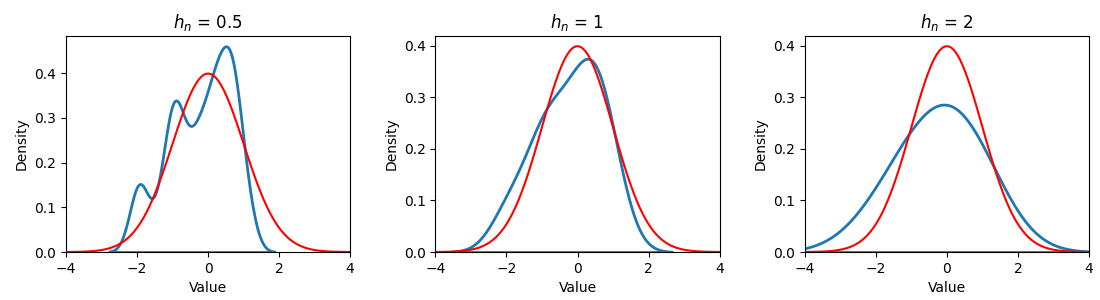
\includegraphics[scale=0.6]{part_kde/figures/normal20}}
		\caption{Нормальное распределение, $n=20$}
		\label{fig:kde_normal20}
	\end{figure}

\begin{figure}[H]
	\centering{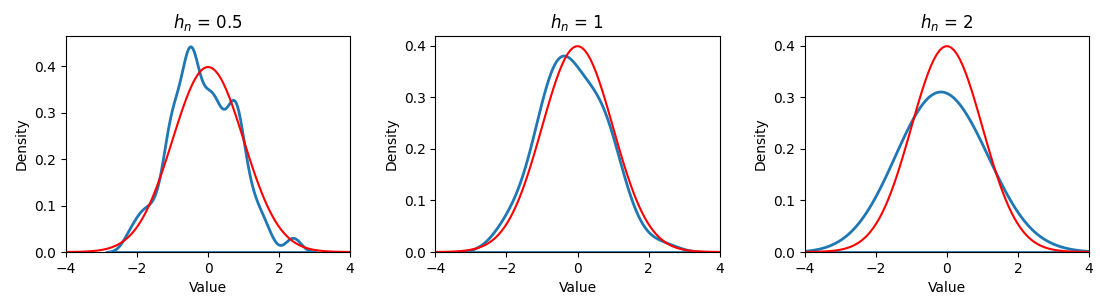
\includegraphics[scale=0.6]{part_kde/figures/normal60}}
		\caption{Нормальное распределение, $n=60$}
		\label{fig:kde_normal60}
	\end{figure}

\begin{figure}[H]
	\centering{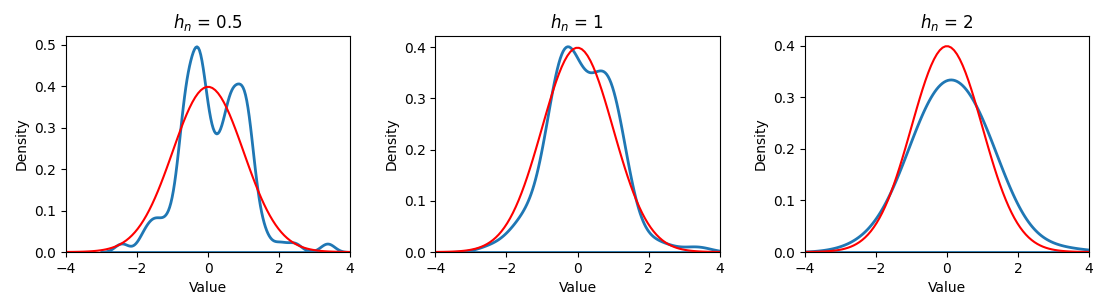
\includegraphics[scale=0.6]{part_kde/figures/normal100}}
		\caption{Нормальное распределение, $n=100$}
		\label{fig:kde_normal100}
	\end{figure}

\begin{figure}[H]
	\centering{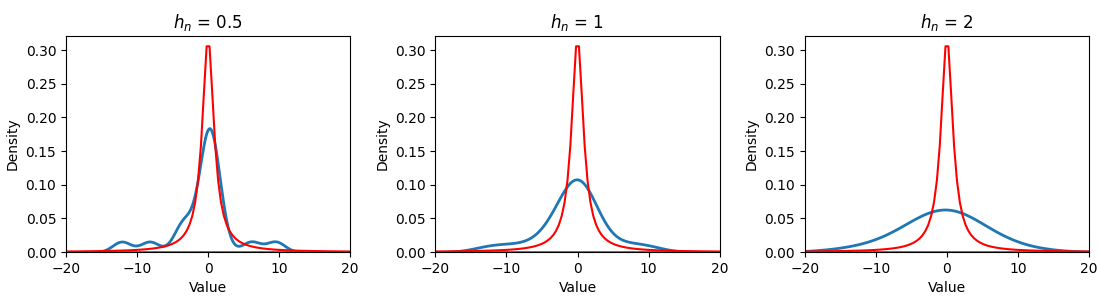
\includegraphics[scale=0.6]{part_kde/figures/cauchy20}}
		\caption{Распределение Коши, $n=20$}
		\label{fig:kde_cauchy20}
	\end{figure}

\begin{figure}[H]
	\centering{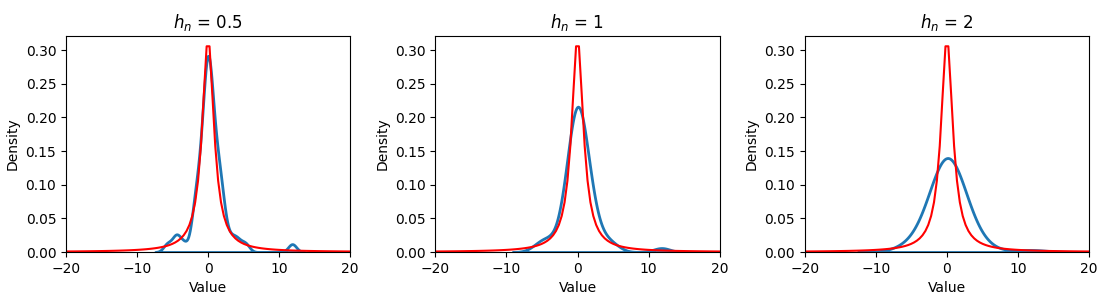
\includegraphics[scale=0.6]{part_kde/figures/cauchy60}}
		\caption{Распределение Коши, $n=60$}
		\label{fig:kde_cauchy60}
	\end{figure}

\begin{figure}[H]
	\centering{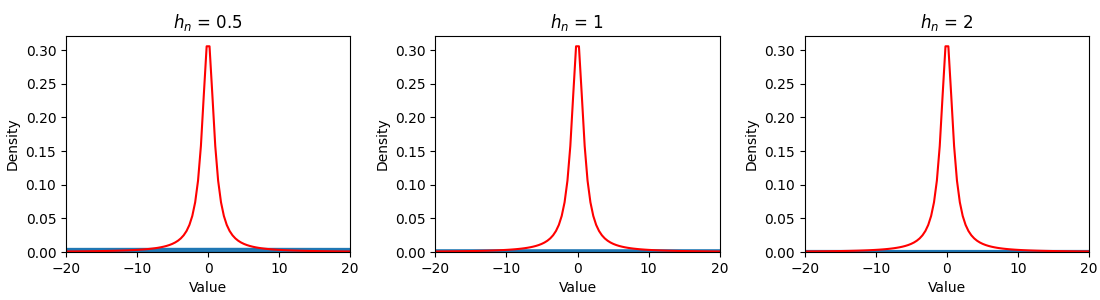
\includegraphics[scale=0.6]{part_kde/figures/cauchy100}}
		\caption{Распределение Коши, $n=100$}
		\label{fig:kde_cauchy100}
	\end{figure}

\begin{figure}[H]
	\centering{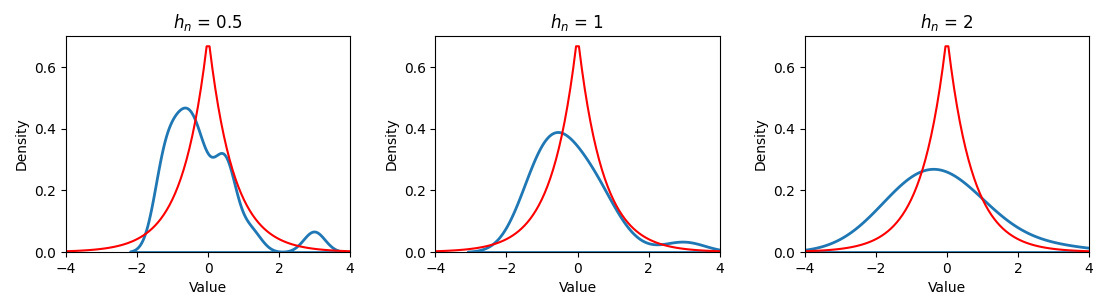
\includegraphics[scale=0.6]{part_kde/figures/laplace20}}
		\caption{Распределение Лапласа, $n=20$}
		\label{fig:kde_laplace20}
	\end{figure}

\begin{figure}[H]
	\centering{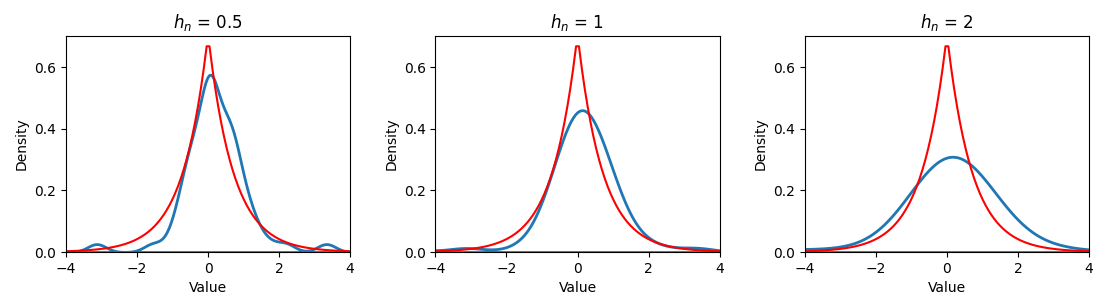
\includegraphics[scale=0.6]{part_kde/figures/laplace60}}
		\caption{Распределение Лапласа, $n=60$}
		\label{fig:kde_laplace60}
	\end{figure}

\begin{figure}[H]
	\centering{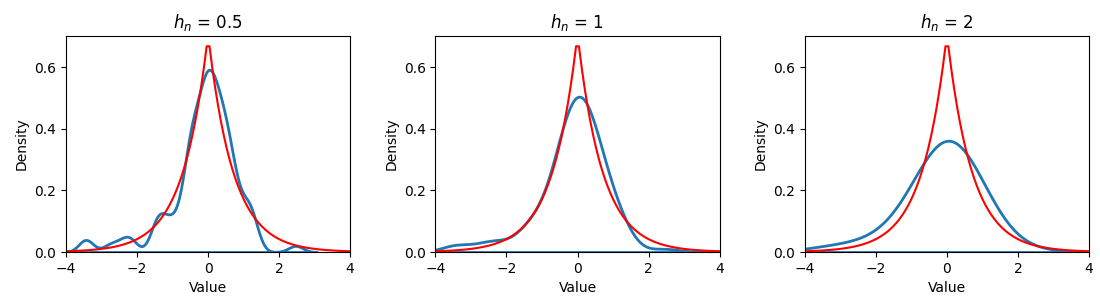
\includegraphics[scale=0.6]{part_kde/figures/laplace100}}
		\caption{Распределение Лапласа, $n=100$}
		\label{fig:kde_laplace100}
	\end{figure}

\begin{figure}[H]
	\centering{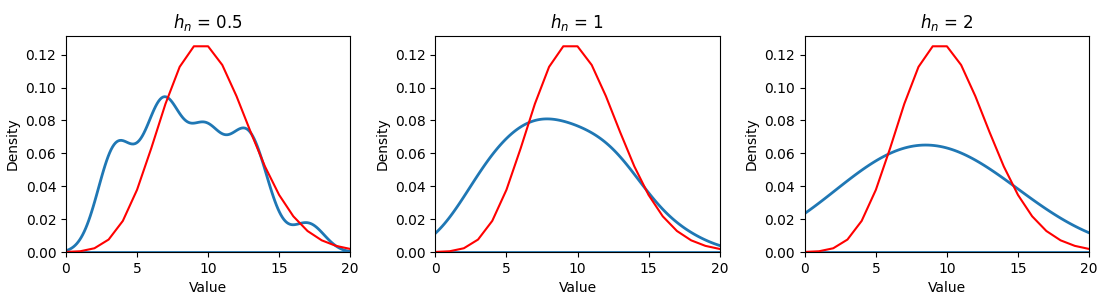
\includegraphics[scale=0.6]{part_kde/figures/poisson20}}
		\caption{Распределение Пуассона, $n=20$}
		\label{fig:kde_poisson20}
	\end{figure}

\begin{figure}[H]
	\centering{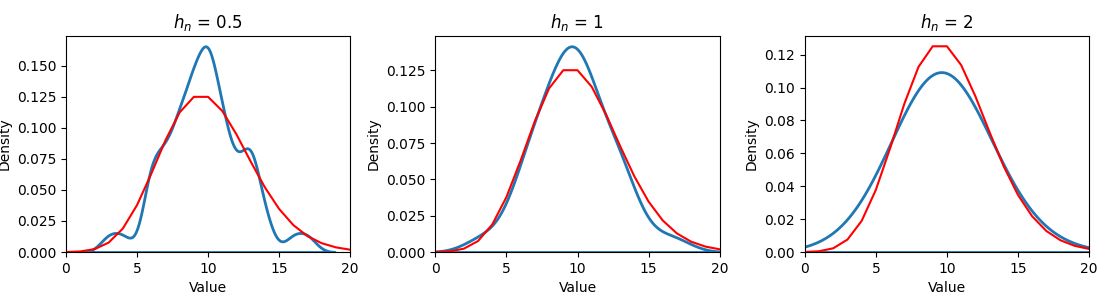
\includegraphics[scale=0.6]{part_kde/figures/poisson60}}
		\caption{Распределение Пуассона, $n=60$}
		\label{fig:kde_poisson60}
	\end{figure}

\begin{figure}[H]
	\centering{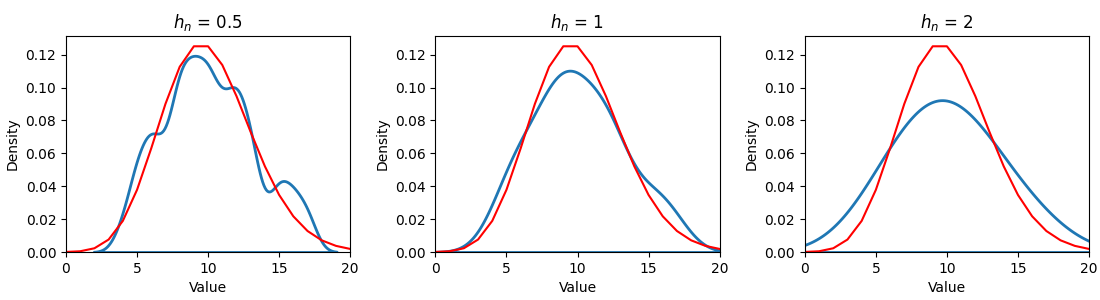
\includegraphics[scale=0.6]{part_kde/figures/poisson100}}
		\caption{Распределение Пуассона, $n=100$}
		\label{fig:kde_poisson100}
	\end{figure}

\begin{figure}[H]
	\centering{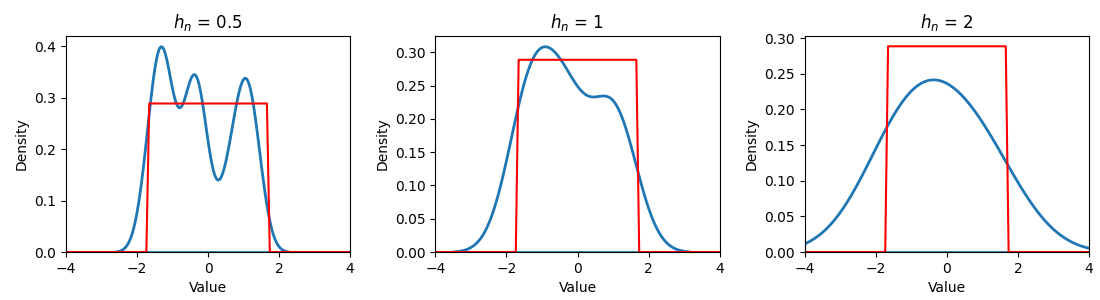
\includegraphics[scale=0.6]{part_kde/figures/uniform20}}
		\caption{Равномерное распределение, $n=20$}
		\label{fig:kde_uniform20}
	\end{figure}

\begin{figure}[H]
	\centering{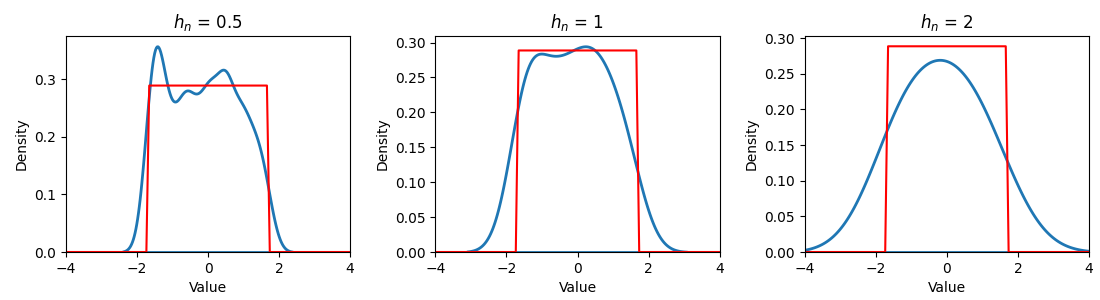
\includegraphics[scale=0.6]{part_kde/figures/uniform60}}
		\caption{Равномерное распределение, $n=60$}
		\label{fig:kde_uniform60}
	\end{figure}

\begin{figure}[H]
	\centering{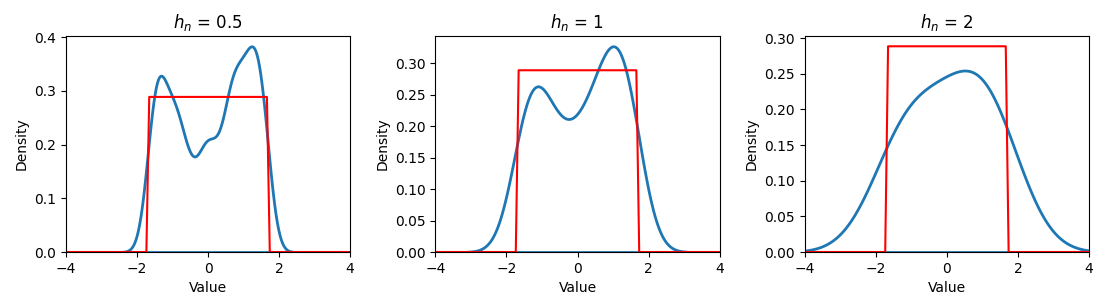
\includegraphics[scale=0.6]{part_kde/figures/uniform100}}
		\caption{Равномерное распределение, $n=100$}
		\label{fig:kde_uniform100}
	\end{figure}